\subsection{问题四：技术演进分析与能力前沿预测}
\begingroup
\setlength{\tabcolsep}{4pt}
\renewcommand{\arraystretch}{1.15}
\clubpenalty=10000
\widowpenalty=10000

\subsubsection{能力度量与数据组织}

前三问比较的是训练后的验证损失，本问转而考察实际评测能力。我们先检查损失较低的模型是否也有较高得分，再分析历史增长中有多少与参数扩张有关，最后估计未来前沿。已有研究讨论过规模增加时的能力涌现\cite{wei2022emergent}，也指出评分方式可能造成看似突然的变化\cite{schaeffer2023mirage}。因此，本文同时保留综合分数和单项任务结果：先统一样本，分层拟合损失与得分，再用规模、时间回归分解增量，以饱和曲线和结构情景预测，并结合任务表现与资源记录讨论限制。

\noindent\textbf{辅助分析说明：} 本问数据整理、绘图与数值核对使用 Codex 辅助，模型为 GPT-5.4（OpenAI，2026-03-05）及 GPT-6 系列（OpenAI，2026-09-03 系列首次发布）\cite{ai_codex54,ai_codex6}。

\textbf{1.综合得分、许可筛选与时间变量}\par\nopagebreak[4]
综合得分取 Open LLM Leaderboard v2 六个维度的等权均值\cite{openllm2025}，记为 $\bar B$，满分为 100。六项分别是 IFEval 指令遵循、BBH 综合推理、MATH Lvl 5 数学、GPQA 研究生级问答、MUSR 多步推理和 MMLU-PRO 专业知识。均分便于比较整体变化，单项分数则用于判断具体能力的不足，两者分别使用。

\Needspace{6\baselineskip}
较近时期的变化使用 C1，长期趋势另以 C3 作参照。时间均按评测记录定义：年度回归取 $t=\text{年份}-2019$，月度前沿使用月中点 \mbox{$t=\text{年份}-2019+(\text{月}-0.5)/12$}，C3 的年度记录放在年中。这样，年度变量用于比较规模与能力的关系，月度变量用于观察较短时间内的前沿变化。

表\ref{tab:p4_funnel}列出样本筛选过程。先保留字段完整的记录，再按许可白名单确定本文讨论的开放权重范围。白名单为 apache-2.0、mit、gpl-3.0、cc-by-4.0、mpl-2.0、bsd-3-clause、cc-by-sa-4.0、openrail，以及 llama2、llama3、llama3.1、llama3.2、llama3.3、gemma。其他和未知许可不进入主样本；列入白名单只表示符合本研究的筛选规则，不代表各许可的使用条件相同。

\begin{table}[!htbp]
\centering
\caption{主样本的形成及模型类型构成}
\label{tab:p4_funnel}
\begin{tabularx}{0.98\textwidth}{@{}
>{\hsize=1\hsize\linewidth=\hsize\raggedright\arraybackslash}X
>{\hsize=0.45\hsize\linewidth=\hsize\centering\arraybackslash}X
>{\hsize=1.55\hsize\linewidth=\hsize\raggedright\arraybackslash}X@{}}
\toprule
数据层次 & 记录数 & 判定依据或构成 \\
\midrule
C1 原始记录 & 4{,}576 & 六维得分均完整；日期覆盖 2024-06 至 2025-03 \\
完整性筛选后 & 4{,}561 & 日期、参数量和六维得分齐备，排除 15 条记录 \\
许可白名单主样本 & 2{,}346 & 以 Hub License 字段匹配许可集合 \\
\midrule
预训练类 & 231 & pretrained 与持续预训练模型 \\
对话及微调类 & 1{,}497 & chat 与领域微调模型 \\
其他类型 & 618 & 包含 611 条合并模型记录和 7 条多模态记录 \\
\bottomrule
\end{tabularx}
\end{table}

表中的三类模型均保留在主样本中，类型只用于分组比较。为观察基础训练与后训练的差异，再分别估计预训练类、对话及微调类的规模和时间系数。C3 的历史记录则按六维得分一致性和参数有效性筛选，没有沿用 C1 的许可白名单，所以长期分析不能看成对同一批开放权重模型的持续追踪。

\textbf{2.从原始评测记录到子任务样本}\par\nopagebreak[4]
细分任务来自 C8，其 1{,}863 个模型目录共含 1{,}958 个 JSON 文件。每个目录优先读取最新文件，解析失败时再回退，最终 1{,}860 个目录取得有效结果，3 个没有可用记录。指标按 acc\_norm、acc、prompt\_level\_loose\_acc、inst\_level\_loose\_acc、exact\_match 的顺序选取，并换算为百分制。规范化模型名称后，与主样本对应的有 964 个目录。由此汇总 BBH 24 项、MATH-Hard 7 项、GPQA 3 项、MUSR 3 项，共 37 项任务，各项有效样本为 961 至 964 个。

C8 与 C1 的分数不能直接混用。前者保留原始指标，后者对汇总得分作了基准调整：GPQA 的随机基线为 0.25，MMLU-PRO 为 0.10，因此原始比例 $s$ 分别变为 $(s-0.25)/0.75$、$(s-0.10)/0.90$。IFEval 还对严格判定下的提示级、指令级结果取平均。本文因此用 C1 比较综合能力，用 C8 比较任务内部的原始表现。

按名称关联后，两套得分的比较见表\ref{tab:p4_c8chk}。C1 中同名的多条记录均保留，因此配对数可能多于 C8 目录数，不能当作独立模型数。六维 Spearman 系数均高于 0.81，多数高于 0.97，说明排序大体相近；但 BBH、GPQA、MUSR 的绝对差较大。排序接近并没有消除任务构成和归一化方式的差别。

\begin{table}[!htbp]
\centering
\caption{原始指标与汇总得分的记录级一致性}
\label{tab:p4_c8chk}
\begin{tabularx}{0.98\textwidth}{@{}
>{\hsize=1.4\hsize\linewidth=\hsize\raggedright\arraybackslash}X
>{\hsize=0.95\hsize\linewidth=\hsize\centering\arraybackslash}X
>{\hsize=0.8\hsize\linewidth=\hsize\centering\arraybackslash}X
>{\hsize=0.8\hsize\linewidth=\hsize\centering\arraybackslash}X
>{\hsize=1.05\hsize\linewidth=\hsize\centering\arraybackslash}X@{}}
\toprule
评测维度 & \makecell{有效配对\\记录数} & \makecell{秩相关\\$\rho$} & \makecell{线性相关\\$r$} & \makecell{平均绝对\\偏差 / 分} \\
\midrule
IFEval & 1{,}896 & 0.987 & 0.987 & 2.88 \\
BBH & 1{,}898 & 0.997 & 0.998 & 21.06 \\
MATH Lvl 5 & 1{,}897 & 0.812 & 0.803 & 3.47 \\
GPQA & 1{,}894 & 0.992 & 0.987 & 23.38 \\
MUSR & 1{,}894 & 0.977 & 0.973 & 30.73 \\
MMLU-PRO & 1{,}896 & 0.998 & 0.998 & 7.56 \\
\bottomrule
\end{tabularx}
\end{table}

\subsubsection{损失与评测得分的分层联系}

要将前三问的损失结果用于解释能力变化，首先需要检验二者的对应关系。设验证损失为 $L$，采用便于比较方向和误差的线性映射：
\begin{equation}
    \bar B = a + b\,L
\end{equation}
采用最小二乘估计该关系。C6 的高可比记录主要来自同模型、同验证集的 Pythia，可与附件 B 对照；中可比记录来自不同模型族和技术报告，验证集并不统一。我们分别拟合这两层，再报告合并样本与 C5 的对照结果，使来源差异能够在结果中体现。

\begin{figure}[!htbp]
\centering
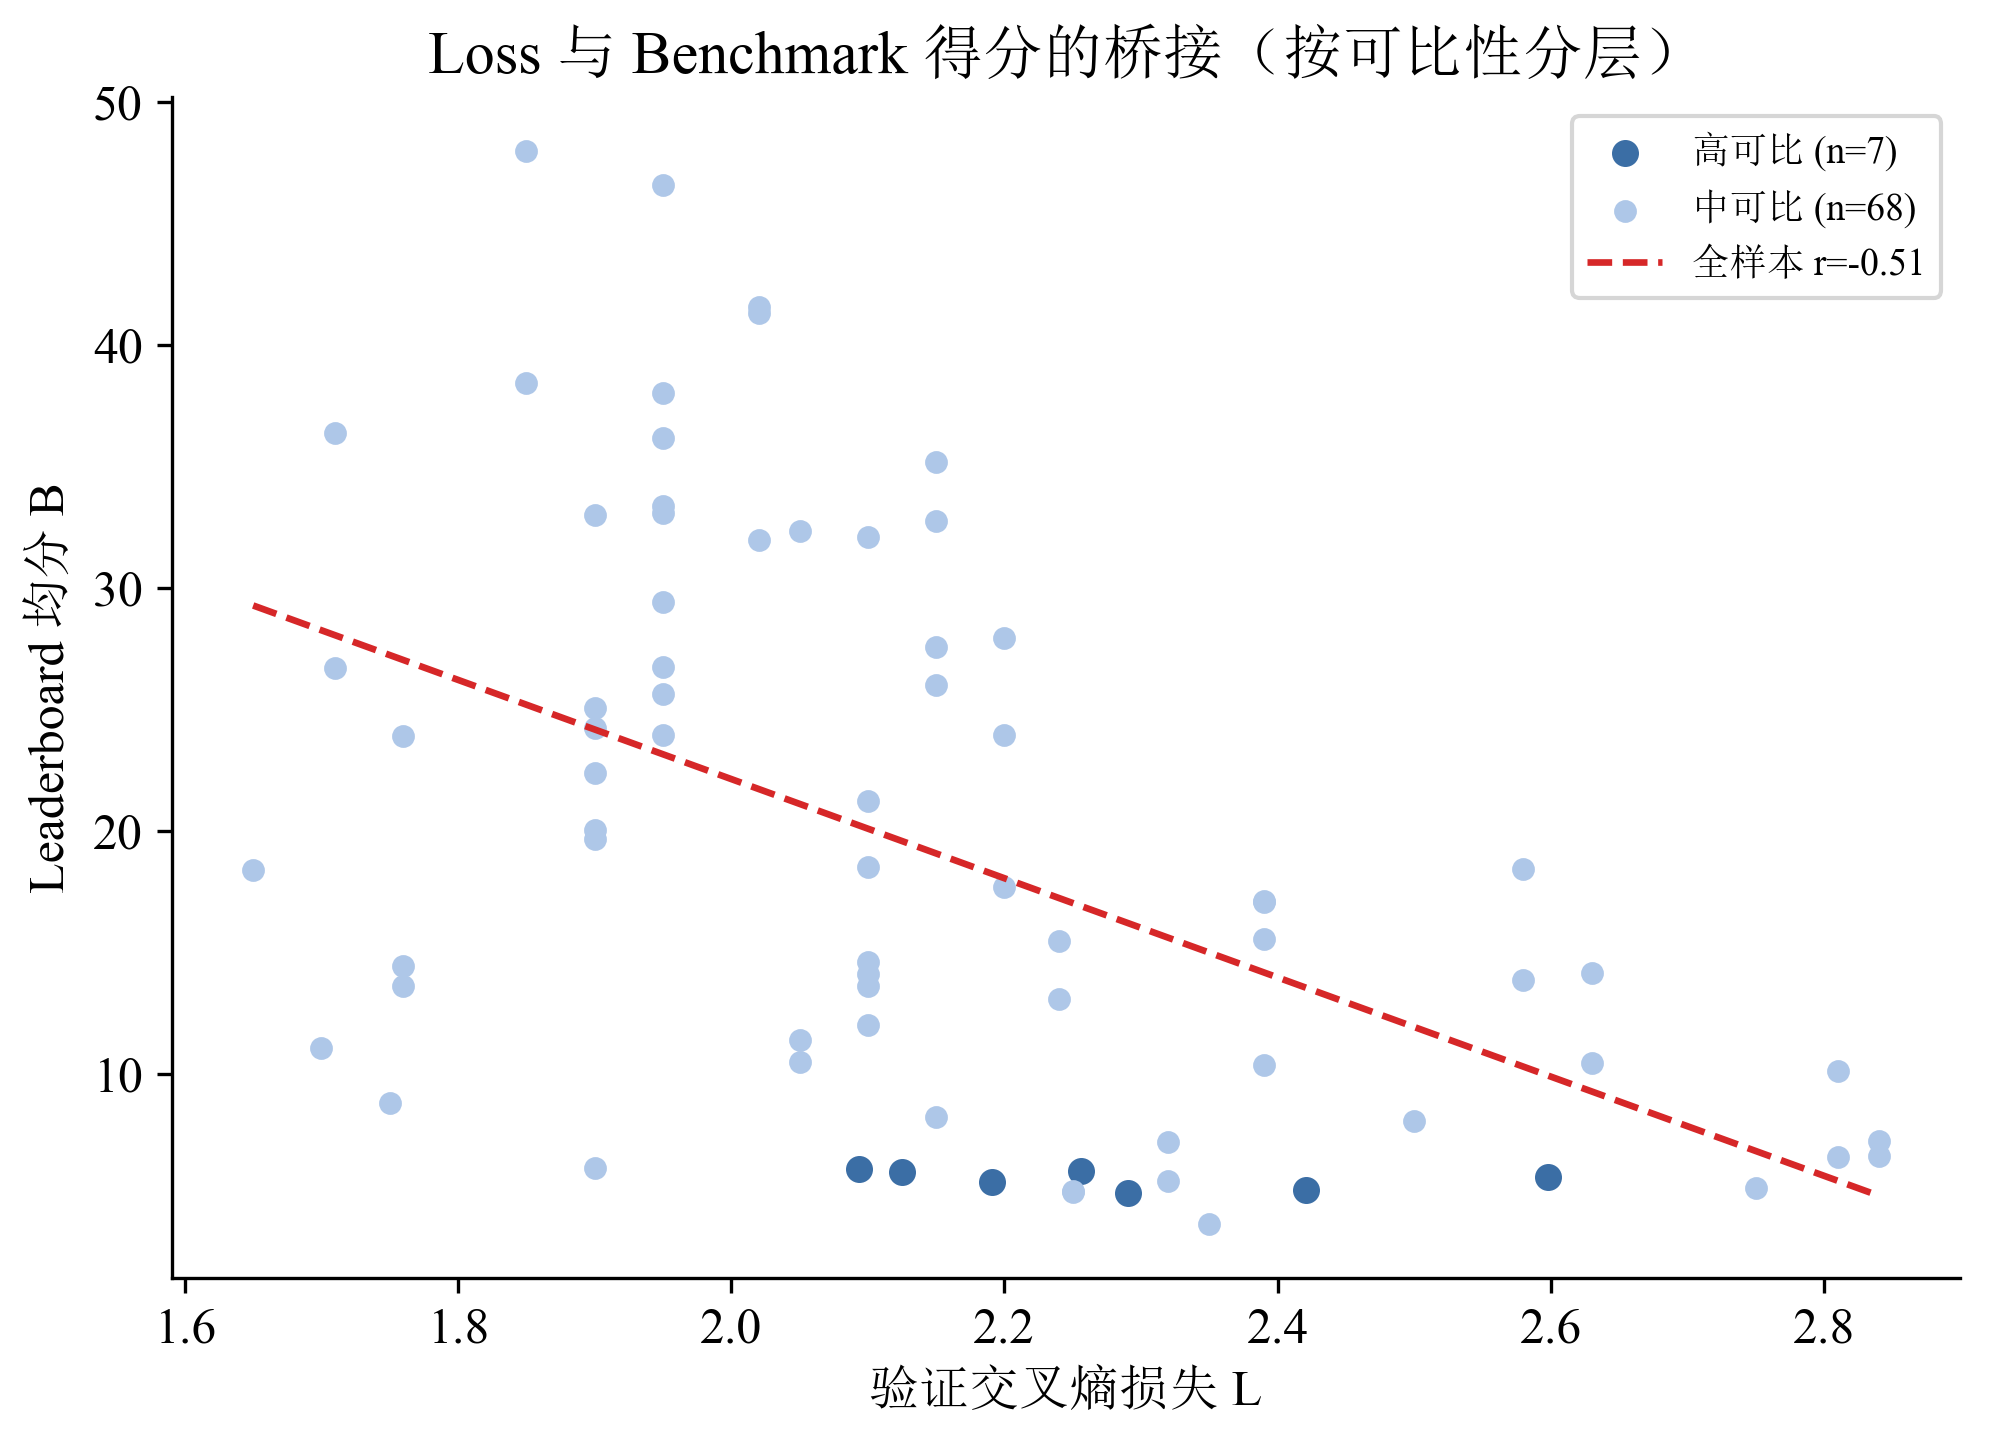
\includegraphics[width=0.98\textwidth]{../求解/问题四/图片/图1_Loss_Benchmark映射.png}
\caption{验证损失与得分的分层关系：点为 C6 记录，线为对应层的最小二乘拟合；两面板纵轴范围不同}
\label{fig:p4_map}
\end{figure}

\begin{table}[!htbp]
\centering
\caption{损失映射的方向、解释度与误差}
\label{tab:p4_bridge}
\begin{tabularx}{0.98\textwidth}{@{}
>{\hsize=1.25\hsize\linewidth=\hsize\raggedright\arraybackslash}X
>{\hsize=0.9375\hsize\linewidth=\hsize\centering\arraybackslash}X
>{\hsize=0.9375\hsize\linewidth=\hsize\centering\arraybackslash}X
>{\hsize=0.9375\hsize\linewidth=\hsize\centering\arraybackslash}X
>{\hsize=0.9375\hsize\linewidth=\hsize\centering\arraybackslash}X@{}}
\toprule
评价量 & \makecell{C6 高可比\\$n=7$} & \makecell{C6 中可比\\$n=68$} & \makecell{C6 合并\\$n=75$} & \makecell{C5 对照\\$n=43$} \\
\midrule
损失斜率 $b$ & $-0.882$ & $-19.185$ & $-20.417$ & $-16.155$ \\
Pearson $r$ & $-0.397$ & $-0.502$ & $-0.510$ & $-0.502$ \\
Spearman $\rho$ & $-0.607$ & $-0.509$ & $-0.549$ & — \\
决定系数 $R^2$ & 0.16 & 0.25 & 0.26 & — \\
MAPE / \% & 5.6 & 57.3 & 67.8 & — \\
\bottomrule
\end{tabularx}
\end{table}

图\ref{fig:p4_map}和表\ref{tab:p4_bridge}显示，损失较低时得分总体较高，但两者并没有形成精确的换算关系。合并样本的 Pearson $r=-0.510$、Spearman $\rho=-0.549$，$R^2$ 只有 0.26，MAPE 为 67.8\%。中可比层验证集不同，低得分又容易放大相对误差。高可比层虽有 5.6\% 的 MAPE，却只有 7 条记录，得分也仅在 $5.07\sim6.06$ 之间，不能据此推断高能力模型同样适用。

因此，这一步只支持损失与能力大体反向变化，不能把前三问的损失改善精确换成能力分，也不能由跨模型相关推断资源调整的因果效果。接下来的历史分解和预测直接使用 Benchmark 得分，以免继续传递这一换算误差。

\subsubsection{规模关系与历史增量分解}

\textbf{1.控制年份后的规模关联}\par\nopagebreak[4]
令 $P_{it}$ 表示模型参数量，单位为十亿参数。对模型记录建立包含规模和时间的回归，并以年份固定效应作对照：
\begin{equation}
    \text{Score}_{it} = b_0 + b_P\log_{10}P_{it} + b_t\,t + \varepsilon_{it}
    \qquad\text{或}\qquad
    \text{Score}_{it} = \alpha_t + b_P\log_{10}P_{it} + \varepsilon_{it}
\end{equation}
控制年份后，$b_P$ 表示参数量扩大十倍时的得分差；控制规模后，$b_t$ 表示每年的得分变化。$\alpha_t$ 用于表示各年的共同差异。上述系数描述条件关联，不能进一步分出数据工程、模型架构或对齐技术各自的因果作用。

主样本中，2024 年有 1{,}588 条，2025 年有 758 条。由于只有两个年份，线性年度变量与年份固定效应在这里可以表示同样的变化，得到相同的规模系数和 $R^2$ 并不意外，也不能当作两次独立验证。图\ref{fig:p4_scale}保留了每年内部的分散情况，表\ref{tab:p4_panel}进一步对照各类模型。

\begin{figure}[!htbp]
\centering
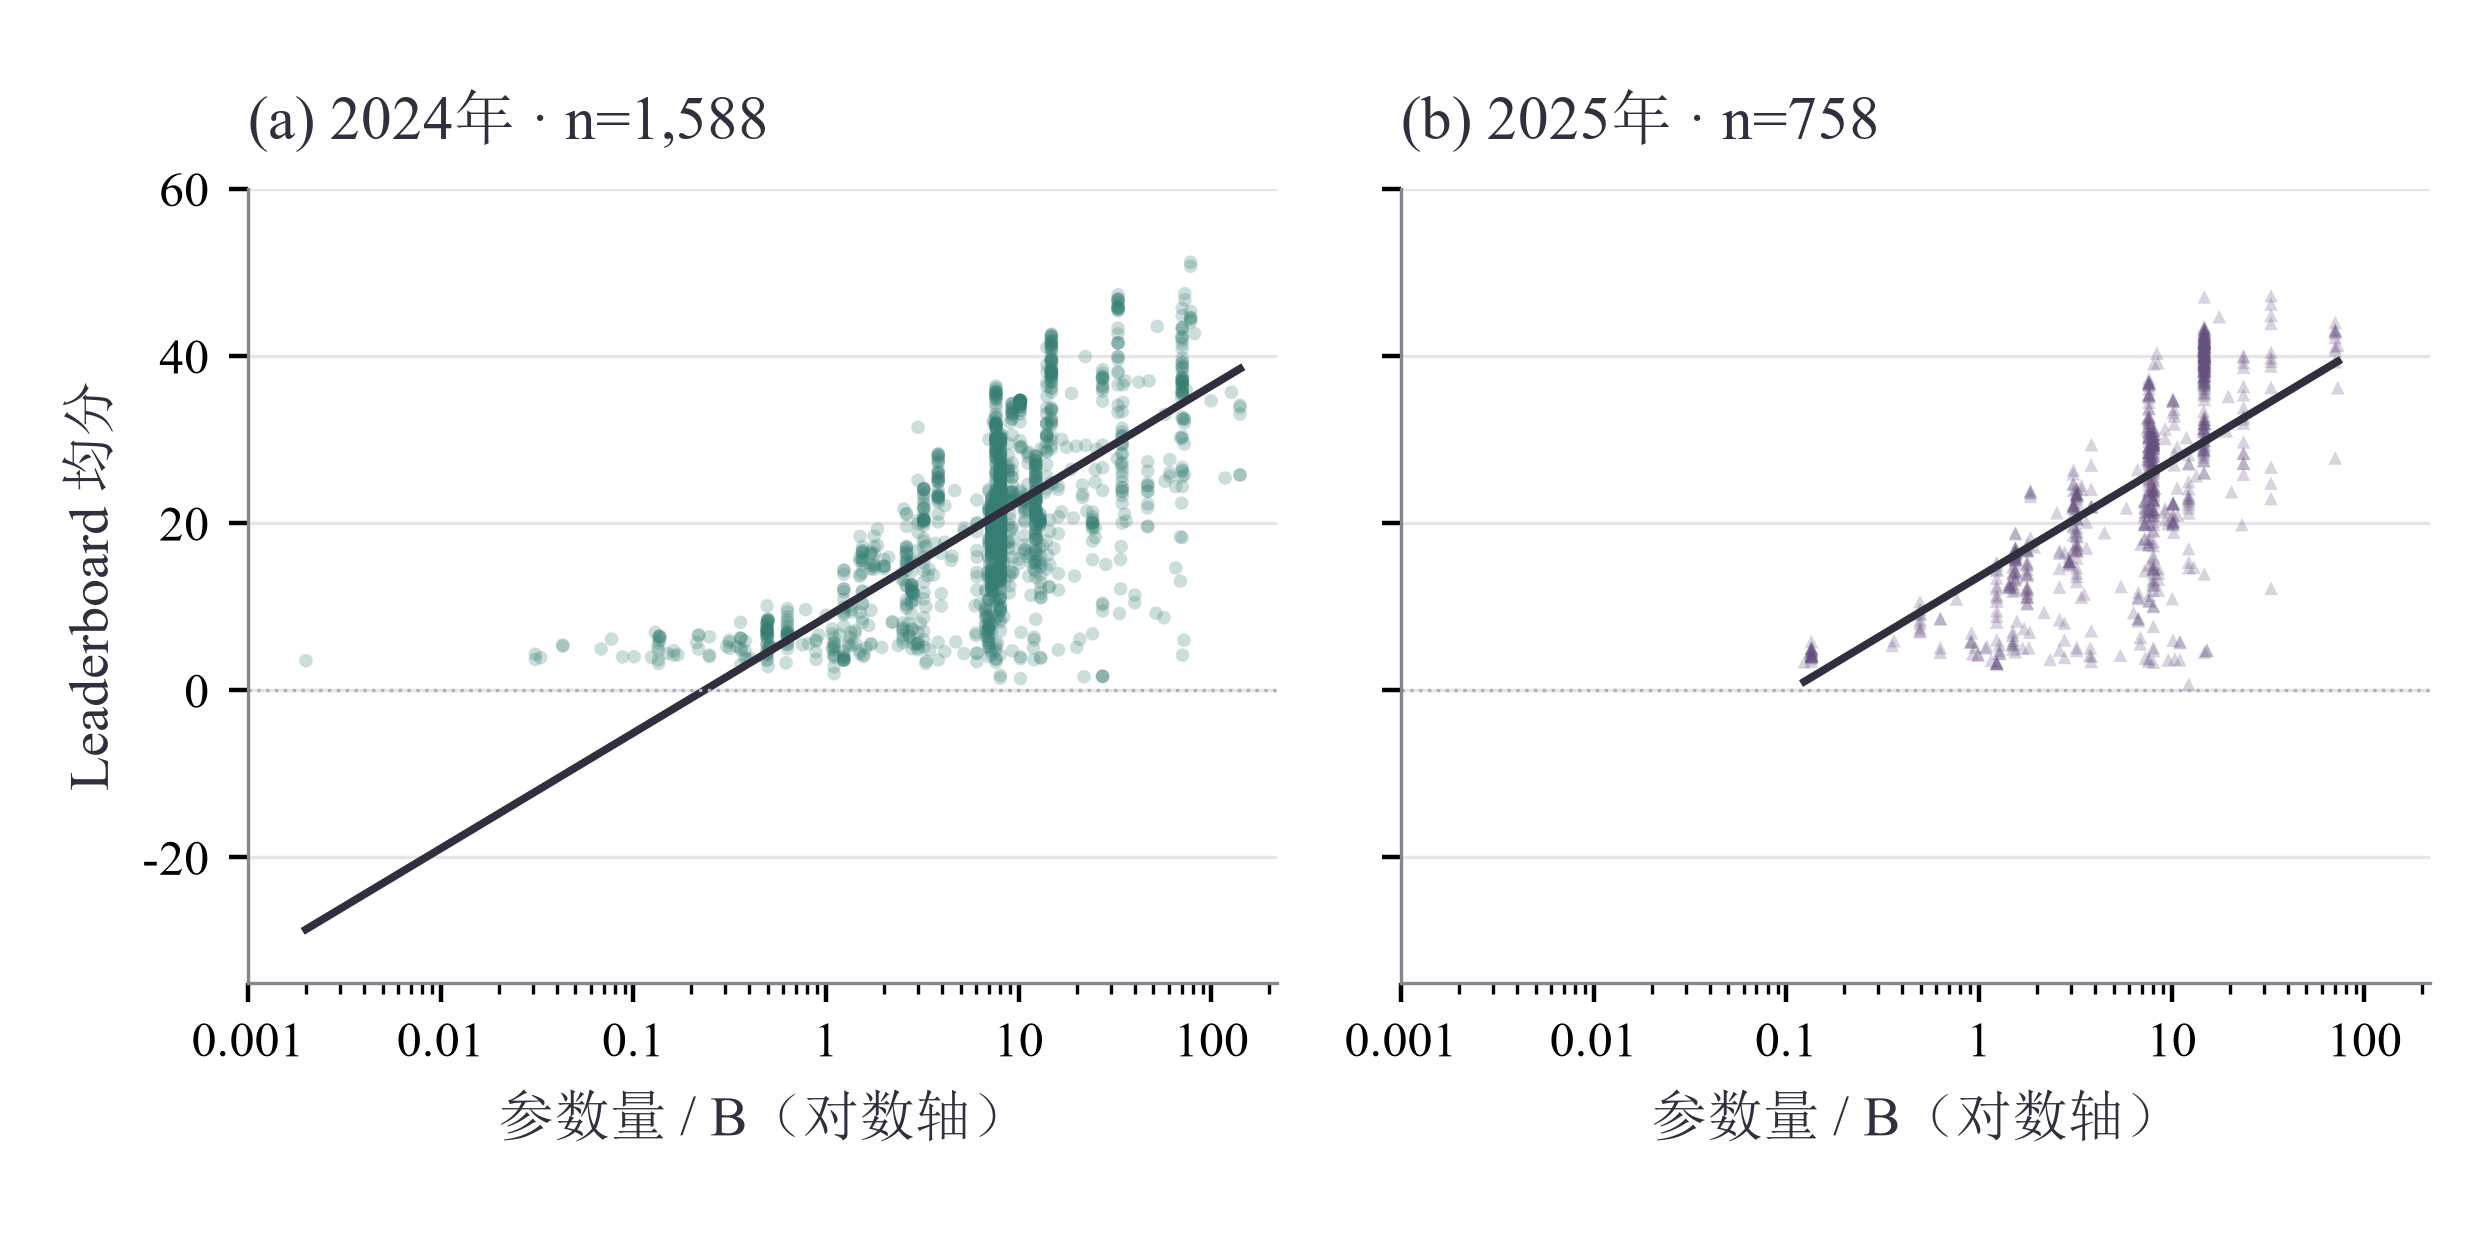
\includegraphics[width=0.98\textwidth]{../求解/问题四/图片/图7_年度规模效应.png}
\caption{按提交年份分组的规模与得分关系：点为主样本记录，直线使用同一规模系数及对应年份效应}
\label{fig:p4_scale}
\end{figure}

\begin{table}[!htbp]
\centering
\caption{全样本与类型子样本的规模、时间系数}
\label{tab:p4_panel}
\begin{tabularx}{0.98\textwidth}{@{}
>{\hsize=2\hsize\linewidth=\hsize\raggedright\arraybackslash}X
>{\hsize=0.6\hsize\linewidth=\hsize\centering\arraybackslash}X
>{\hsize=0.85\hsize\linewidth=\hsize\centering\arraybackslash}X
>{\hsize=0.85\hsize\linewidth=\hsize\centering\arraybackslash}X
>{\hsize=0.7\hsize\linewidth=\hsize\centering\arraybackslash}X@{}}
\toprule
样本与时间设定 & $n$ & \makecell{$b_P$\\分/十倍参数} & \makecell{$b_t$\\分/年} & $R^2$ \\
\midrule
主样本，年份固定效应 & 2{,}346 & 13.842 & — & 0.475 \\
主样本，线性年度项 & 2{,}346 & 13.842 & 4.844 & 0.475 \\
预训练类，线性年度项 & 231 & 6.414 & 1.552 & 0.460 \\
对话及微调类，线性年度项 & 1{,}497 & 14.853 & 4.680 & 0.484 \\
\bottomrule
\end{tabularx}
\end{table}

全样本的规模、年度系数分别为 13.842、4.844；预训练类为 6.414、1.552；对话及微调类为 14.853、4.680。不同类型的差异说明，解释回归时需要考虑样本构成。这里没有同一模型微调前后的受控比较，故不能直接认定微调提高了参数利用效率。此外，线性式在极小参数端可能预测负分，本节只用它概括规模关系和核算增量，不把它当作适用于全部规模的有界评分函数。

\textbf{2.长周期与近端窗口的贡献核算}\par\nopagebreak[4]
为量化历史增量，采用 shift-share 分解，将前沿得分变化拆为规模项与剩余项：
\begin{equation}
    \Delta F = \underbrace{b_P\,\Delta\log_{10}P_{\text{frontier}}}_{\text{规模扩张贡献}}
    + \underbrace{\left[\Delta F - b_P\,\Delta\log_{10}P_{\text{frontier}}\right]}_{\text{非规模技术进步贡献}}
\end{equation}
非规模项按总增量减去规模项计算，既可能包含技术改进，也会吸收样本更替、未观测因素和测量差异。将两项各自除以 $\Delta F$，便得到对应占比。

长期与近期采用不同的前沿定义。C3 以年度累计最高分表示 $F$，用当年保留记录的最大参数量代表规模，两者未必来自同一模型。C1 则取每月前 $1\%$ 得分均值，并使用该前列组中的最大参数量，比较首月到峰值月的变化。因此，两种占比分别对应不同时间尺度，不能合并求平均。

清理 C3 时发现 13 条记录的 Average 与六维均分相差超过 5 分，故将其排除。最大差约 42.3 分，来自 GPT-3 175B：Average 为 50.0，六维均分为 7.67。清理后，长期回归得到 $b_P=14.10$、$b_t=3.30$、$R^2=0.42$。2019 至 2025 年，累计前沿从 5.00 增至 52.08，总增量 47.08 分；规模项对应 23.77 分，非规模项为 23.31 分，占 50.5\% 和 49.5\%。由于历史评测来源仍有差异，这组结果主要用于比较长期量级。

\begin{figure}[!htbp]
\centering
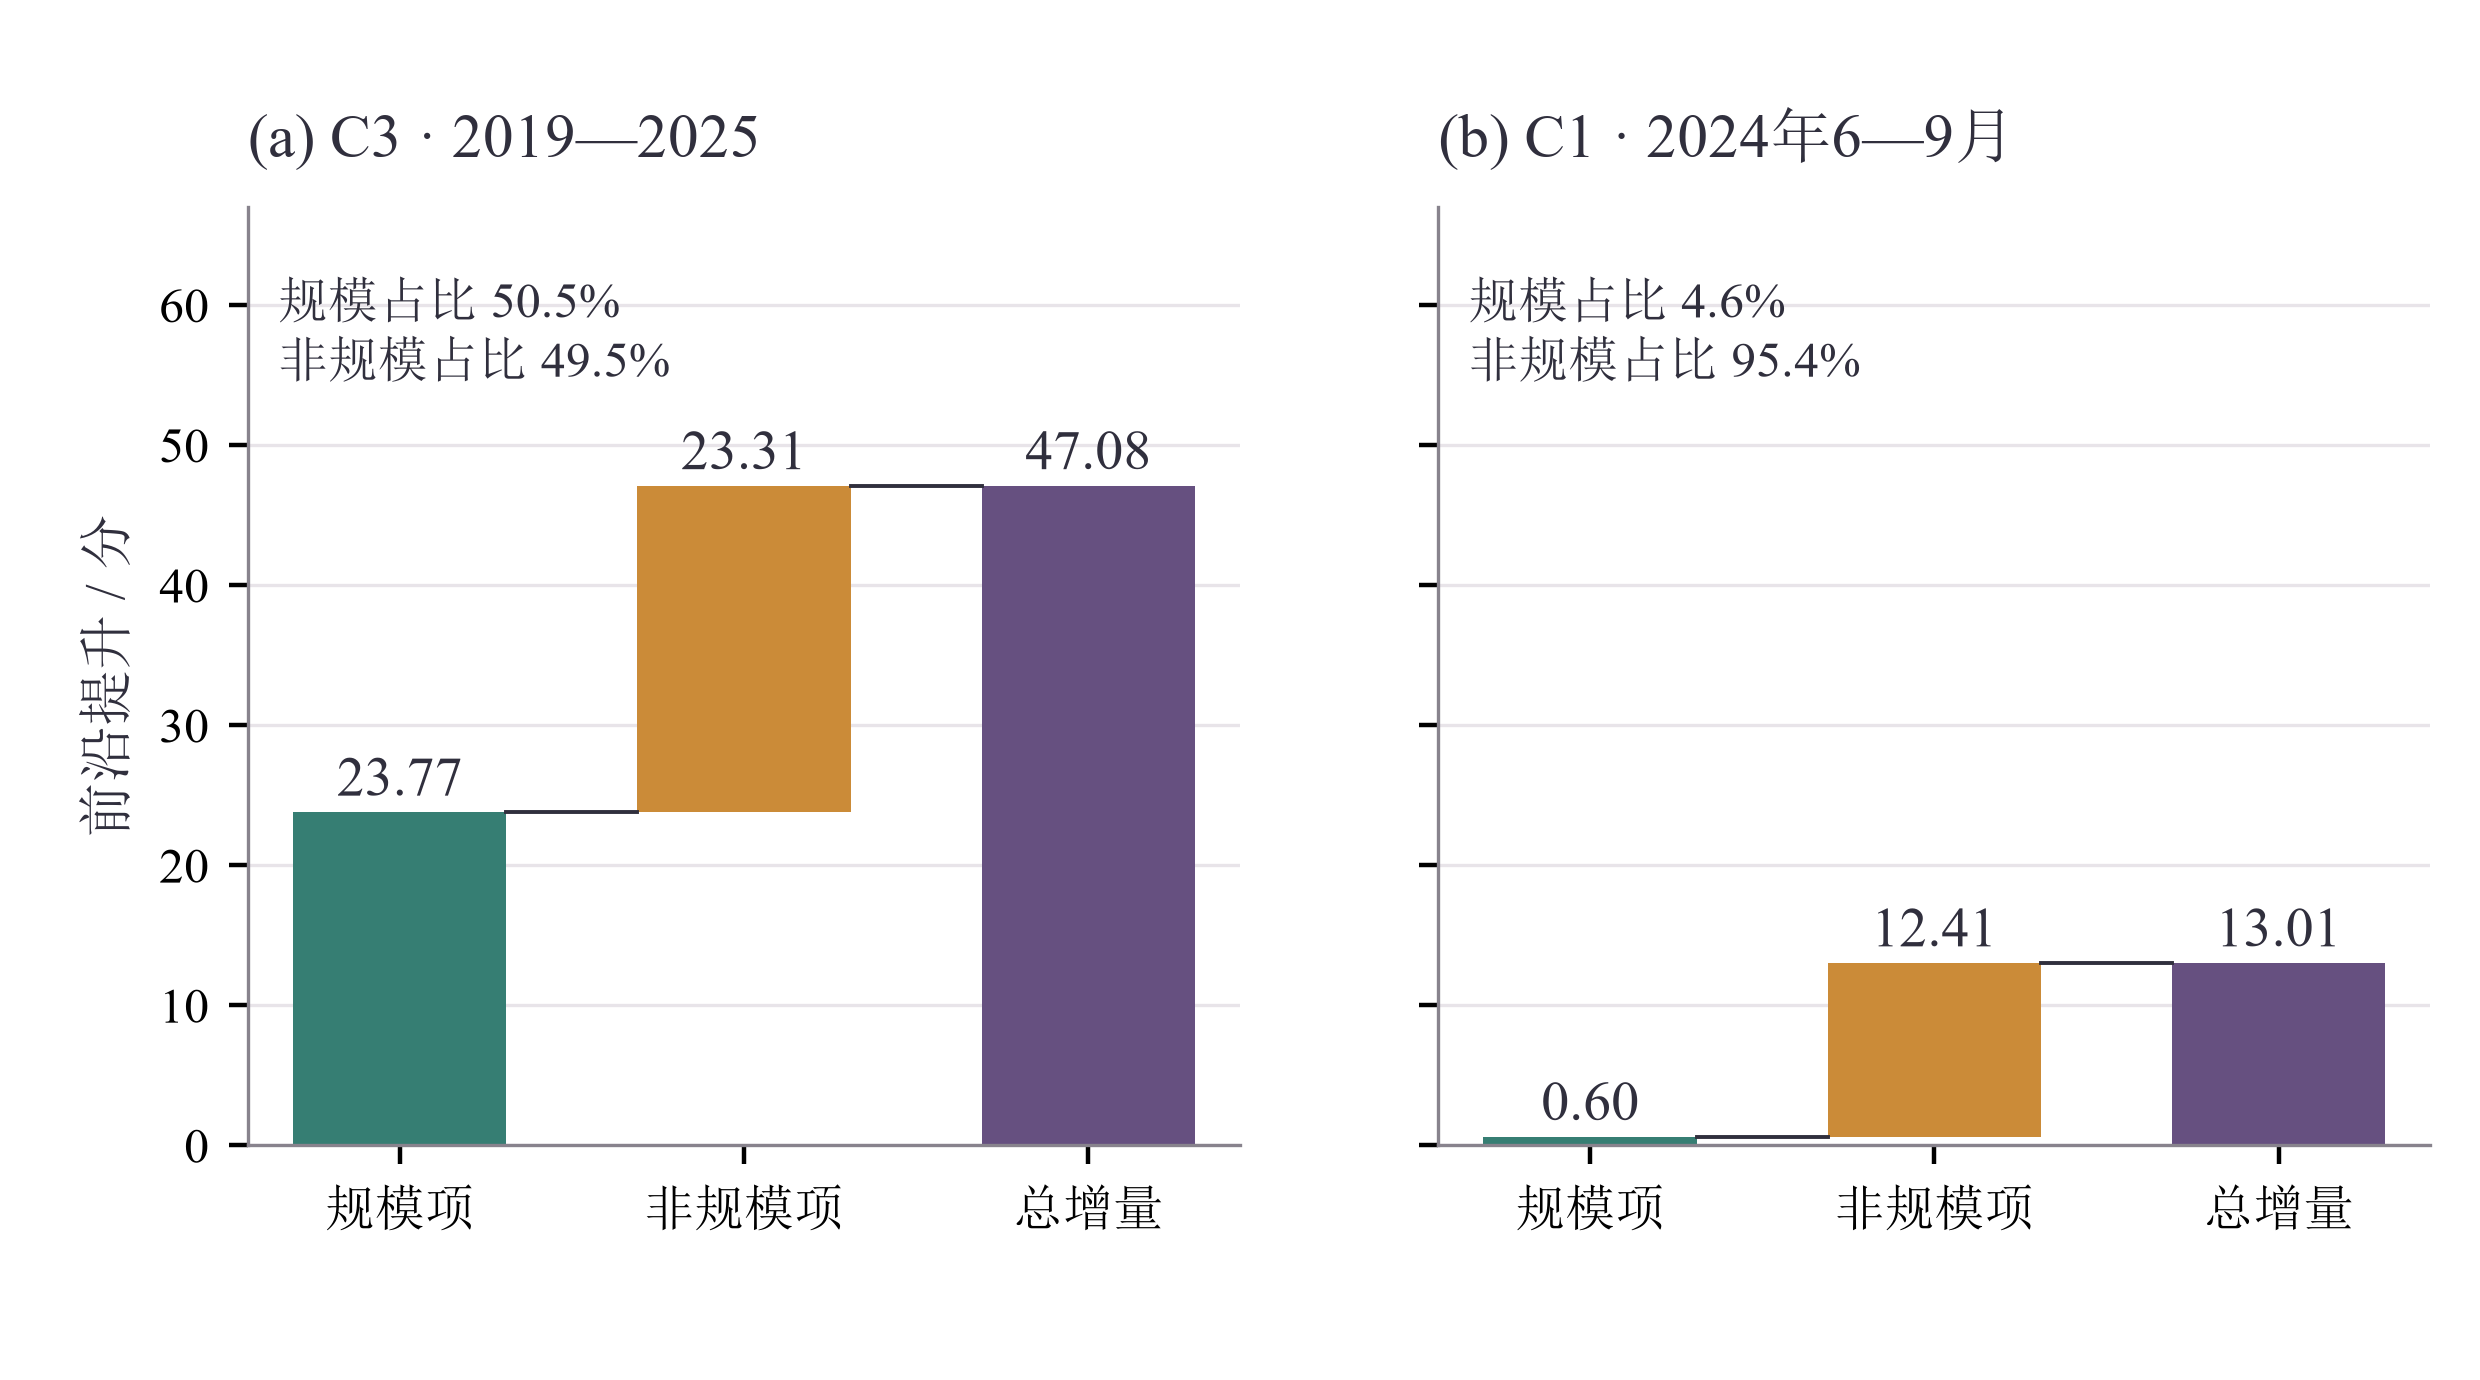
\includegraphics[width=0.98\textwidth]{../求解/问题四/图片/图2_规模时间分解.png}
\caption{两个时间窗口的前沿增量分解：规模项与非规模项相加为总增量；非规模项为分解后的剩余部分}
\label{fig:p4_decomp}
\end{figure}

\Needspace{6\baselineskip}
再看评测框架一致的 C1。2024 年 6 月至 9 月，前沿从 37.99 增至 51.00，而前列组最大参数量只由 70.6B 增至 78.0B，即 $\Delta\log_{10}P=0.043$。分解得到规模项 0.60 分、非规模项 12.41 分，占 4.6\%、95.4\%。图\ref{fig:p4_decomp}表明，这一短窗口的大部分增长不能由参数扩张解释；但其余部分不能直接归为某一种算法作用，也不能将该比例推广到整年或未来。

\subsubsection{前沿曲线与条件预测}

\textbf{1.饱和曲线及重抽样区间}\par\nopagebreak[4]
为预测前沿，将 C3 在 2019 至 2023 年的年度累计最高分，与 C1 月度前 $1\%$ 均值的累计最大值连接，共得到 14 个点。每月前列组人数按记录数的 $1\%$ 向下取整，最少取 1 个。采用 logistic 函数描述逐渐放缓的增长，并限制其上界不超过 100：
\begin{equation}
    F(t) = \frac{K}{1+e^{-r(t-t_0)}},\qquad K \text{ 为饱和上界},\ r \text{ 为增长率},\ t_0 \text{ 为拐点}
\end{equation}
估计结果为 $K=56.61$、$r=2.523$、$t_0=5.11$，拟合 $R^2=0.975$。随后对残差作 600 次 bootstrap 重抽样，用成功重拟合预测值的第 5、第 95 百分位组成 $90\%$ 区间。这反映的是既定曲线下的抽样波动，尚未覆盖评测标准和未来技术路径改变带来的全部不确定性。

算力增长放缓情景以“增速减半”实现：
\begin{equation}
    F_{\text{slow}}(t)=K\left[1+e^{-r(\min(t,t_h)-t_0)}\right]^{-1},\qquad t_h \text{ 为增速减半时刻}
\end{equation}

\textbf{2.基于规模和年度系数的结构情景}\par\nopagebreak[4]
为考察不预设短期饱和时的变化，利用规模和年度系数作结构外推：
\begin{equation}
    \hat F(t+\Delta) = F(t) + \left[b_P\,\Delta\log_{10}P + b_t\right]\cdot\Delta
\end{equation}
式中，$\Delta$ 为向前预测的年数，$\Delta\log_{10}P$ 为假设的\emph{年均}参数对数增量。设置三种条件进行比较：基准情景保持规模不变并延续 $b_t$；放缓情景同样固定规模，但把 $b_t$ 减半；扩容情景则令规模每年增加 0.3 个数量级，同时保留 $b_t$。其中放缓幅度是对非规模增长的假设，并不是从算力增速估计出的传导关系。

\begin{figure}[!htbp]
\centering
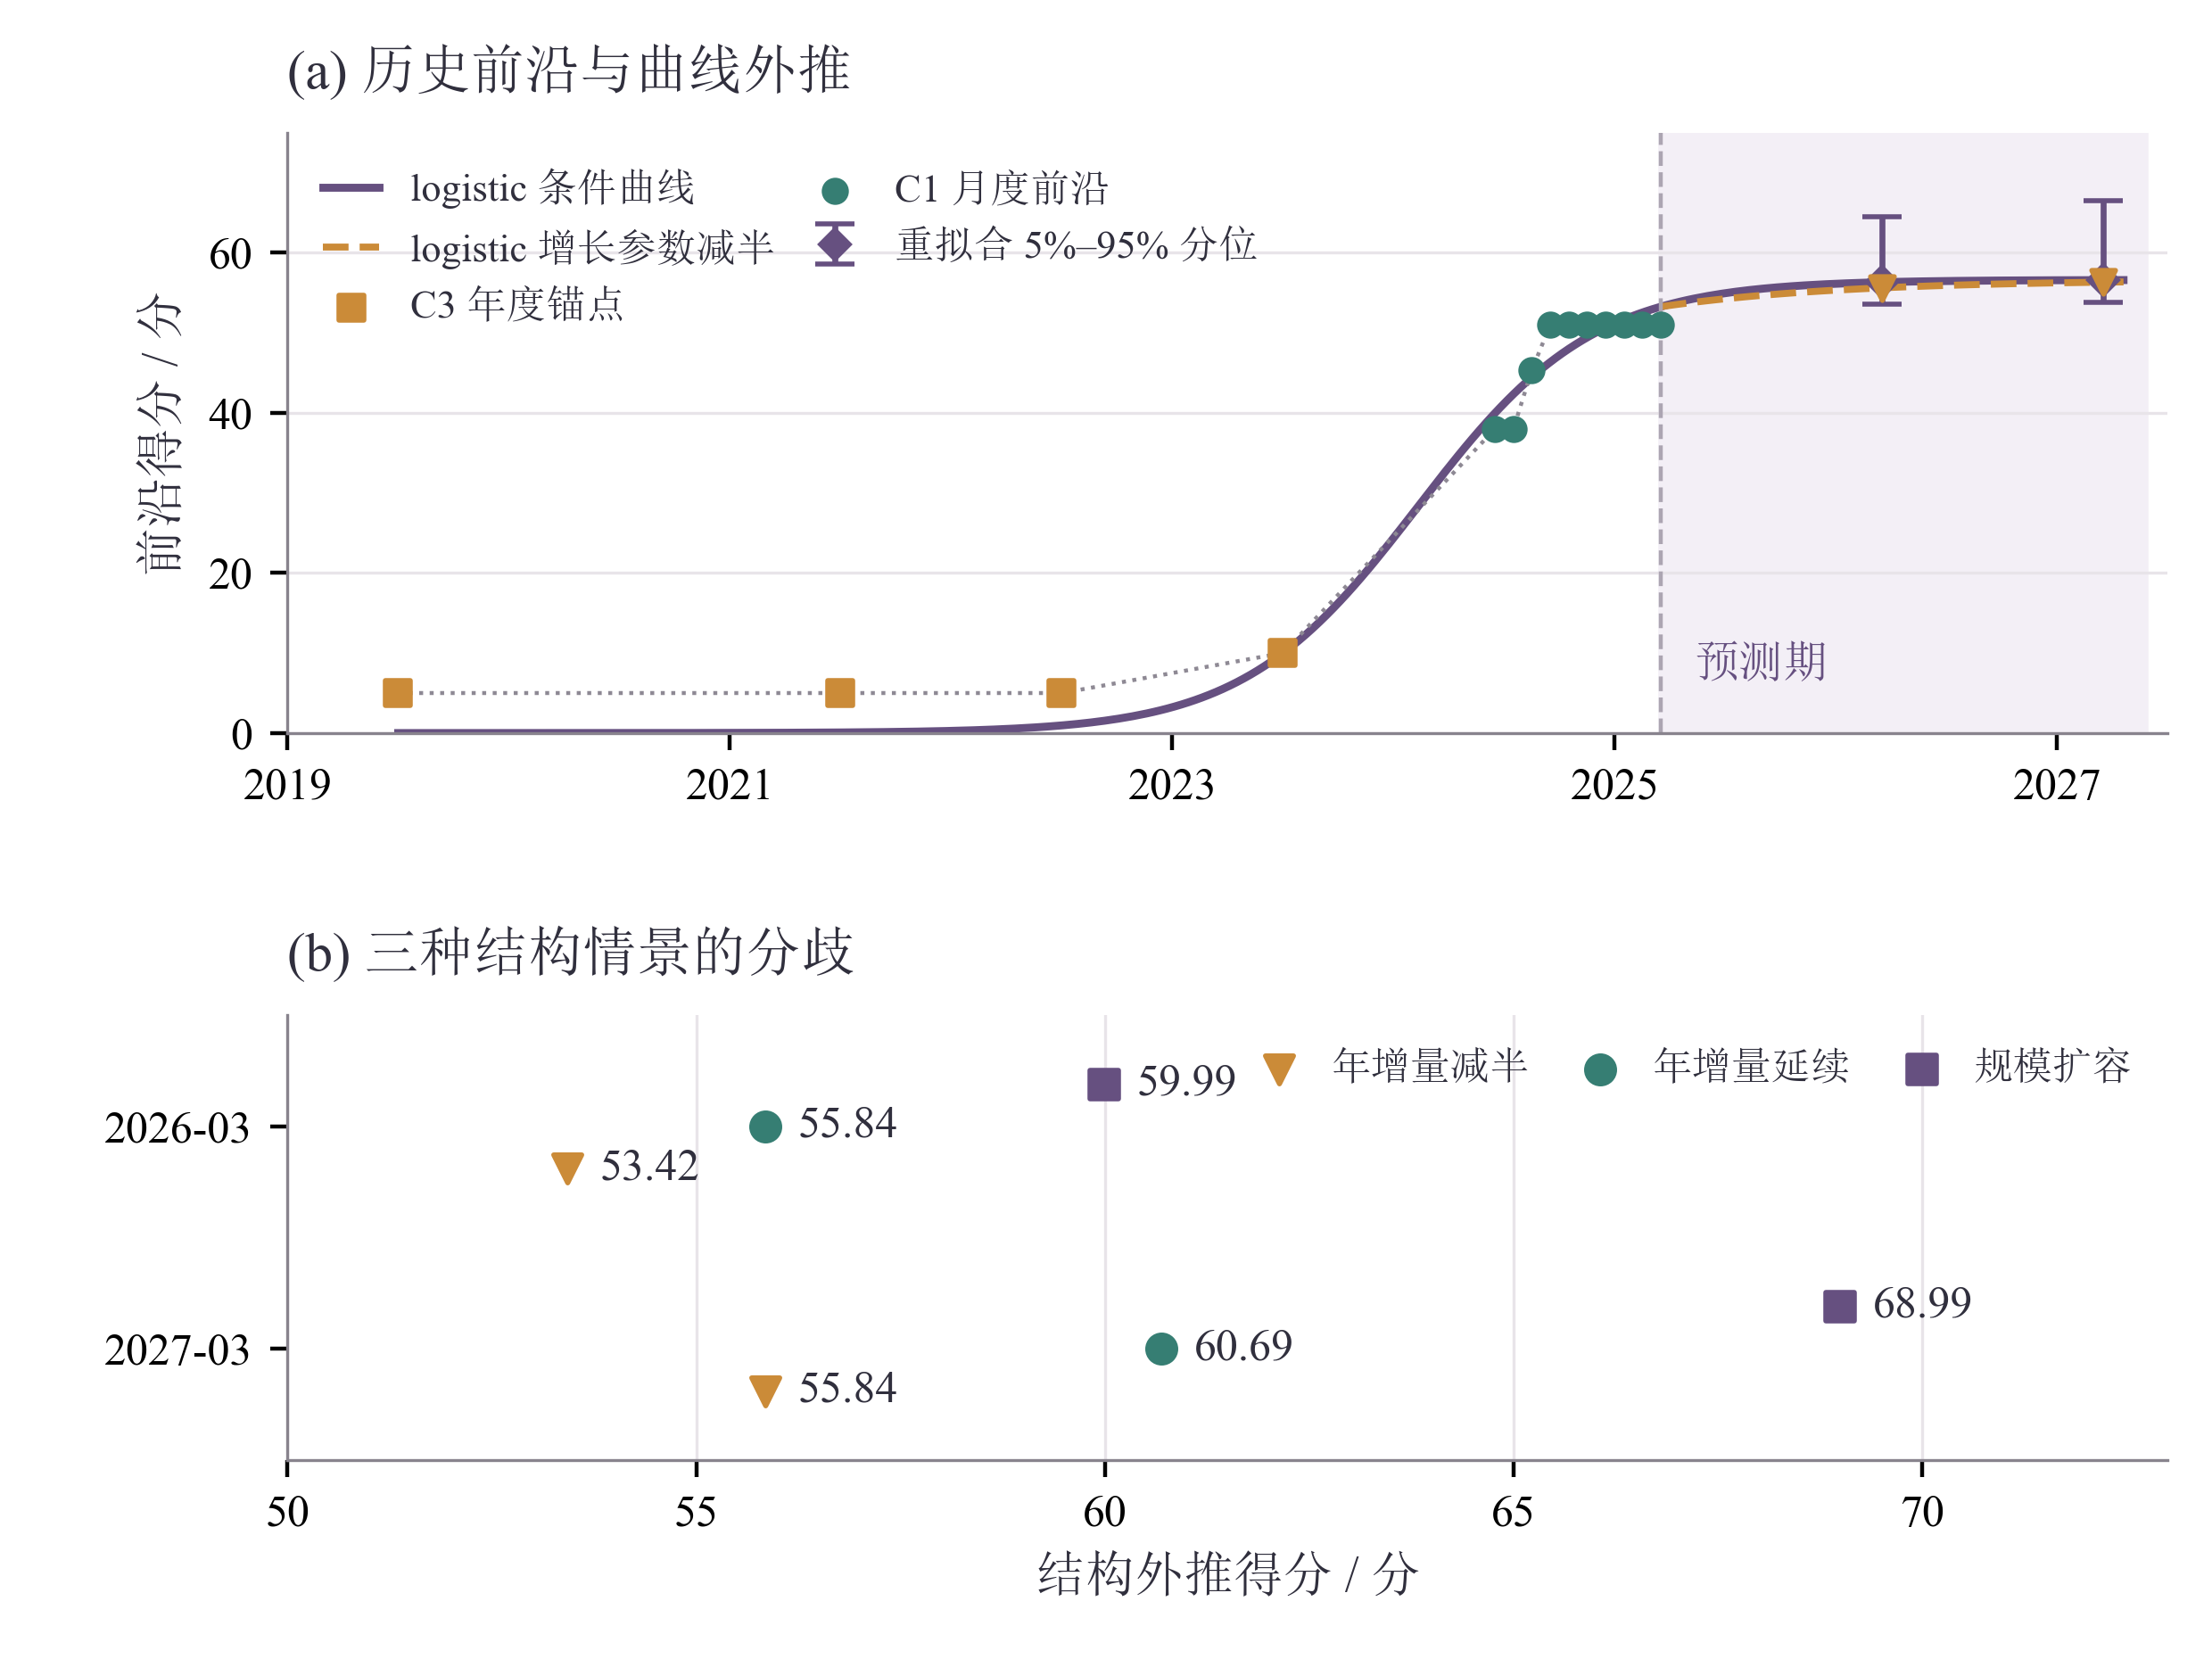
\includegraphics[width=0.98\textwidth]{../求解/问题四/图片/图3_能力前沿预测.png}
\caption{历史前沿与条件预测：上图误差棒为两个预测时点的 $90\%$ bootstrap 区间，下图为结构情景点值}
\label{fig:p4_frontier}
\end{figure}

\begin{table}[!htbp]
\centering
\caption{以 2025 年 3 月数据为基点的能力前沿预测}
\label{tab:p4_frontier}
\begin{tabularx}{0.98\textwidth}{@{}>{\raggedright\arraybackslash}X >{\centering\arraybackslash}X >{\centering\arraybackslash}X@{}}
\toprule
预测口径 & \makecell{前瞻 12 个月\\2026-03} & \makecell{前瞻 24 个月\\2027-03} \\
\midrule
logistic 点预测 & 56.33 & 56.59 \\
bootstrap 第 5 百分位 & 53.62 & 53.75 \\
bootstrap 第 95 百分位 & 64.52 & 66.52 \\
logistic 增速减半 & 53.27 & 53.27 \\
\midrule
结构外推：规模持平 & 55.84 & 60.69 \\
结构外推：非规模增速减半 & 53.42 & 55.84 \\
结构外推：每年扩容 0.3 dex & 59.99 & 68.99 \\
\bottomrule
\end{tabularx}
\end{table}

预测从附件的观测截止时点出发，基点位于 2025 年 3 月，12、24 个月后分别为 2026 年 3 月和 2027 年 3 月。表\ref{tab:p4_frontier}中，logistic 基准预测约为 56.3、56.6 分，$90\%$ 区间为 $[53.62,64.52]$、$[53.75,66.52]$。结构模型的三种情景分别落在 $53.42\sim59.99$ 和 $55.84\sim68.99$ 分，向外取整可概括为 $53\sim60$、$55\sim69$ 分。这一范围来自不同情景的点预测，含义不同于置信区间。

两种预测的主要差别见图\ref{fig:p4_frontier}：饱和曲线在两期之间几乎不再上升，结构基准则假设年度增量继续存在。结构放缓情景得到 53.42、55.84 分，仍有增长，只是速度降低。C1 可比观测约为 10 个月，而前瞻已是其 $1.2\sim2.4$ 倍，早期 C3 又存在评分差异。因此，高拟合度不能代替未来检验，上述数值应与评分体系和情景假设一同使用。

\subsubsection{从综合前沿到具体任务瓶颈}

\textbf{1.六维能力的分布差异}\par\nopagebreak[4]
综合分数还不能说明各项能力是否同时提高。图\ref{fig:p4_distribution}展开六维分布，表\ref{tab:p4_task}列出中位数、前列均值和最高分，使整体水平与领先水平能够同时比较。距满分差值按 $100-\text{最优得分}$ 计算，只表示当前评分上的差距，不能当作一定可以实现的提升量。

\begin{figure}[!htbp]
\centering
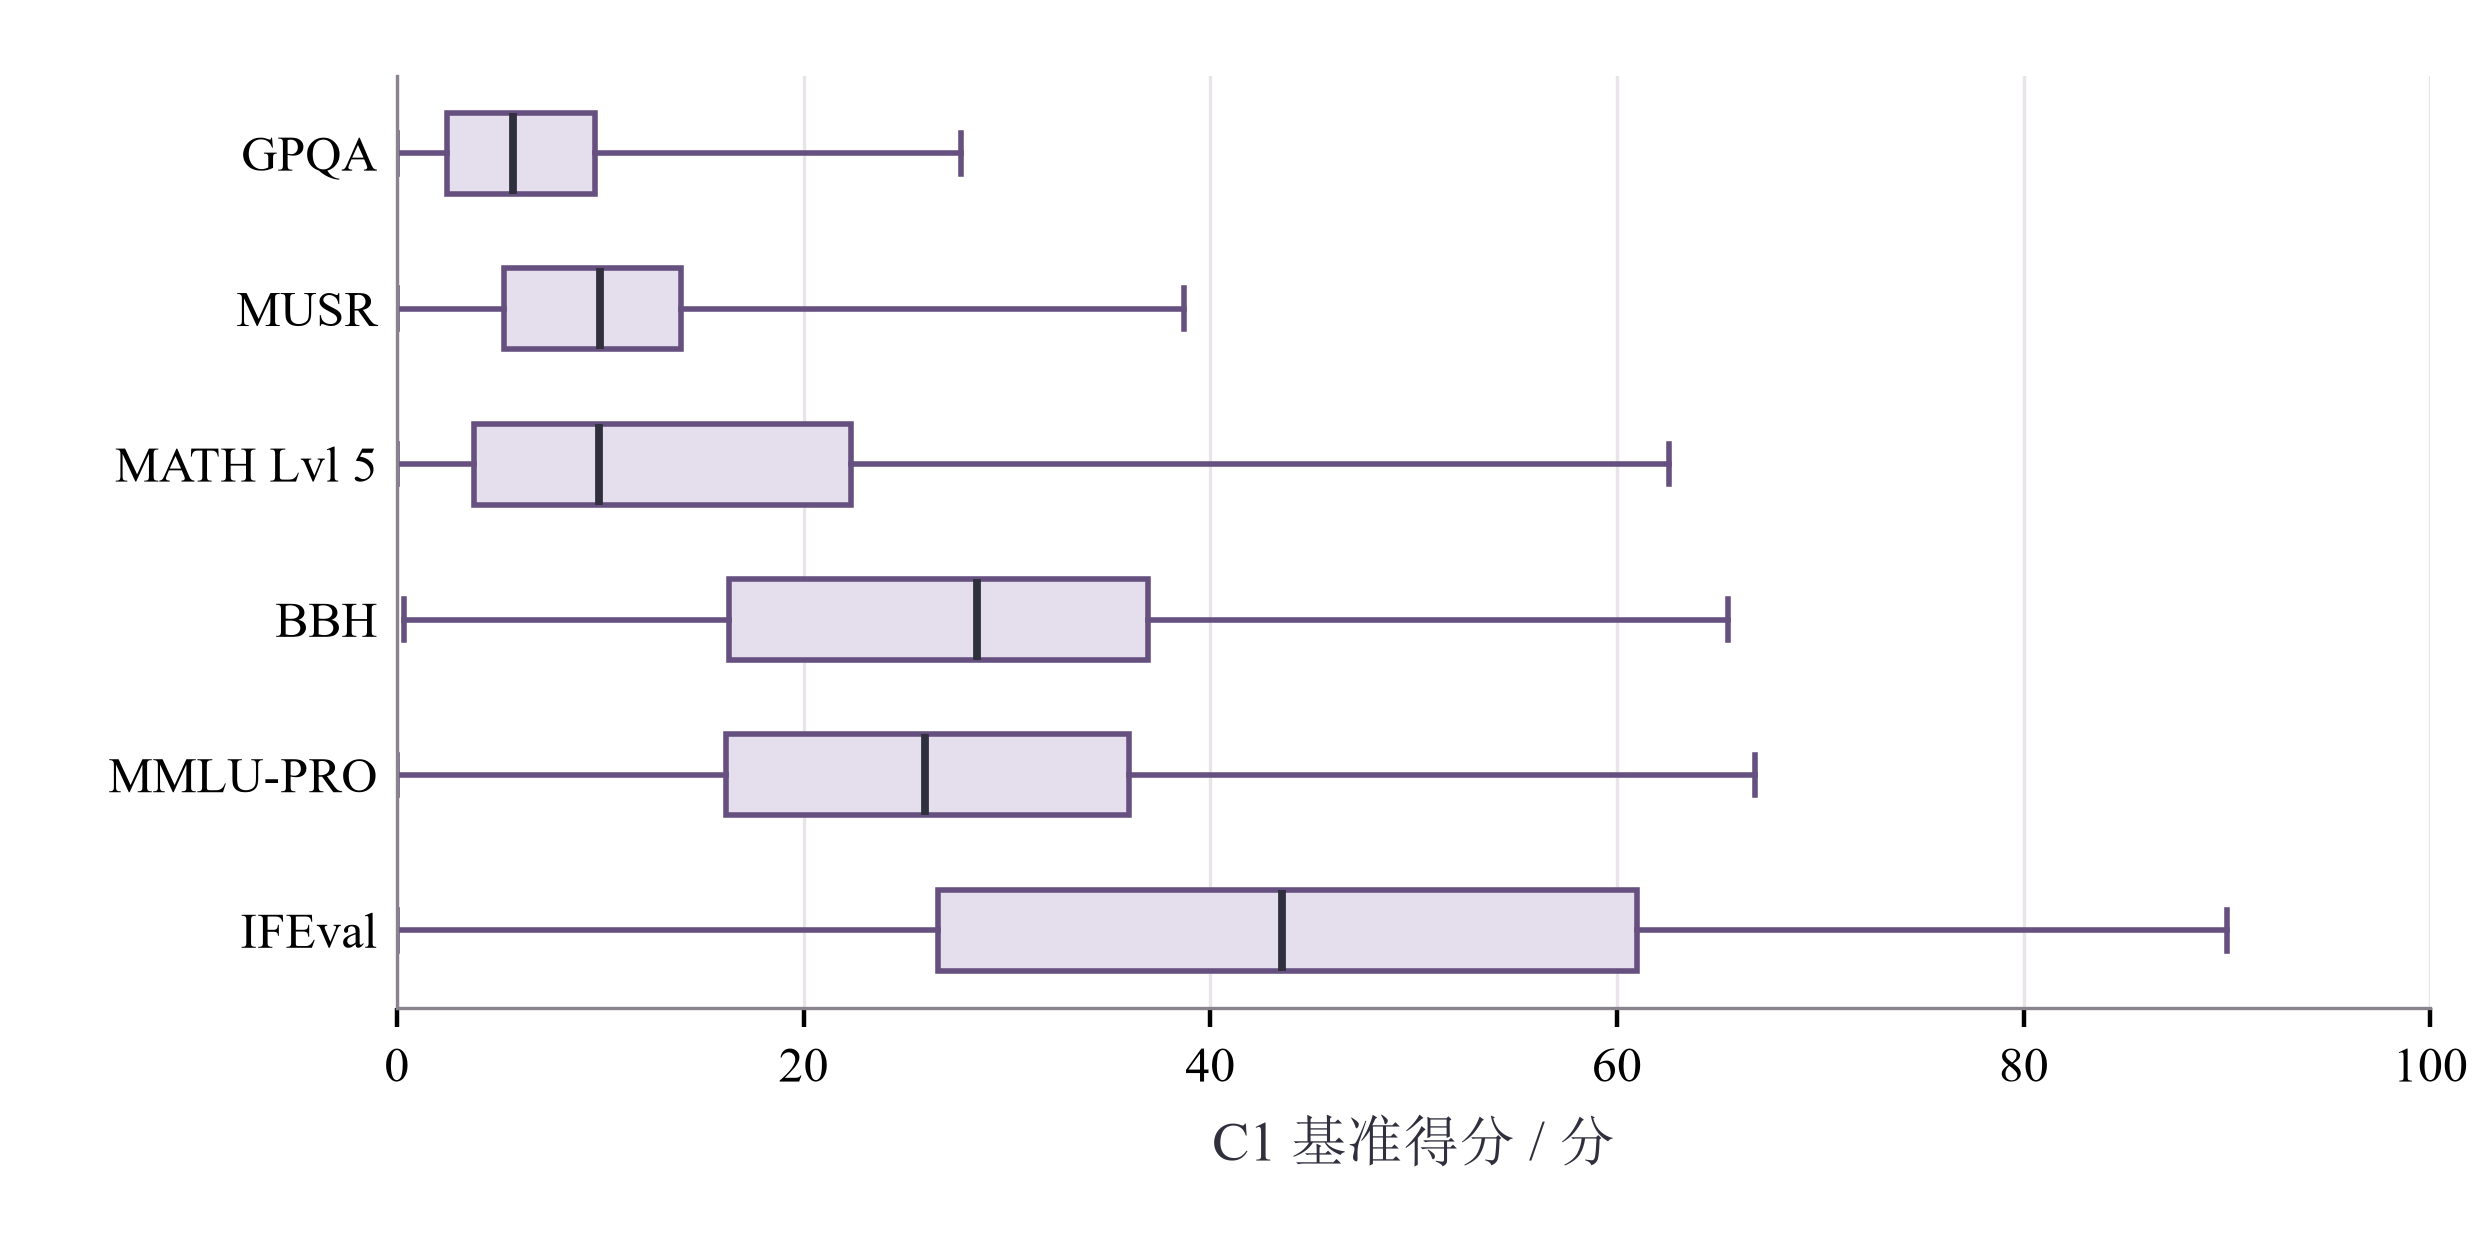
\includegraphics[width=0.98\textwidth]{../求解/问题四/图片/图6_六维能力分布.png}
\caption{主样本的六维能力分布：每维 $n=2{,}346$，箱体为第 25 至第 75 百分位，箱内线为中位数，须线为最小值至最大值}
\label{fig:p4_distribution}
\end{figure}

\begin{table}[!htbp]
\centering
\caption{六维能力的总体水平与前沿差距}
\label{tab:p4_task}
\begin{tabularx}{0.98\textwidth}{@{}
>{\hsize=1.3\hsize\linewidth=\hsize\raggedright\arraybackslash}X
>{\hsize=0.85\hsize\linewidth=\hsize\centering\arraybackslash}X
>{\hsize=1.05\hsize\linewidth=\hsize\centering\arraybackslash}X
>{\hsize=0.9\hsize\linewidth=\hsize\centering\arraybackslash}X
>{\hsize=0.9\hsize\linewidth=\hsize\centering\arraybackslash}X@{}}
\toprule
任务维度 & 中位数 & 前 $1\%$ 均值 & 最优得分 & \makecell{距满分差值\\/ 分} \\
\midrule
GPQA & 5.70 & 22.80 & 27.74 & 72.3 \\
MUSR & 9.97 & 28.06 & 38.69 & 61.3 \\
MATH Lvl 5 & 9.93 & 58.02 & 62.54 & 37.5 \\
BBH & 28.52 & 59.95 & 65.47 & 34.5 \\
MMLU-PRO & 25.98 & 55.26 & 66.80 & 33.2 \\
IFEval & 43.51 & 84.45 & 89.98 & 10.0 \\
\bottomrule
\end{tabularx}
\end{table}

IFEval 最高为 89.98，离满分仅 10.0 分，但中位数仍为 43.51，因此只能说少数领先模型得分较高，不能说整个样本接近饱和。GPQA、MUSR 最高分别为 27.74、38.69，中位数更低，是比较明显的薄弱项。数学的情况也有分化：MATH Lvl 5 最高为 62.54，中位数只有 9.93，说明前沿改善尚未普遍体现在大多数模型上。

\textbf{2.原始子任务中的瓶颈位置}\par\nopagebreak[4]
再把 C8 的 37 个子任务按类别展开，见图\ref{fig:p4_task}。每项同时画出中位数、前 $5\%$ 均值和最高分，分别观察普通样本、前列组和单项前沿。表\ref{tab:p4_sub}列出距满分差值最大的六项，中文名称与图中对应。

\begin{figure}[!htbp]
\centering
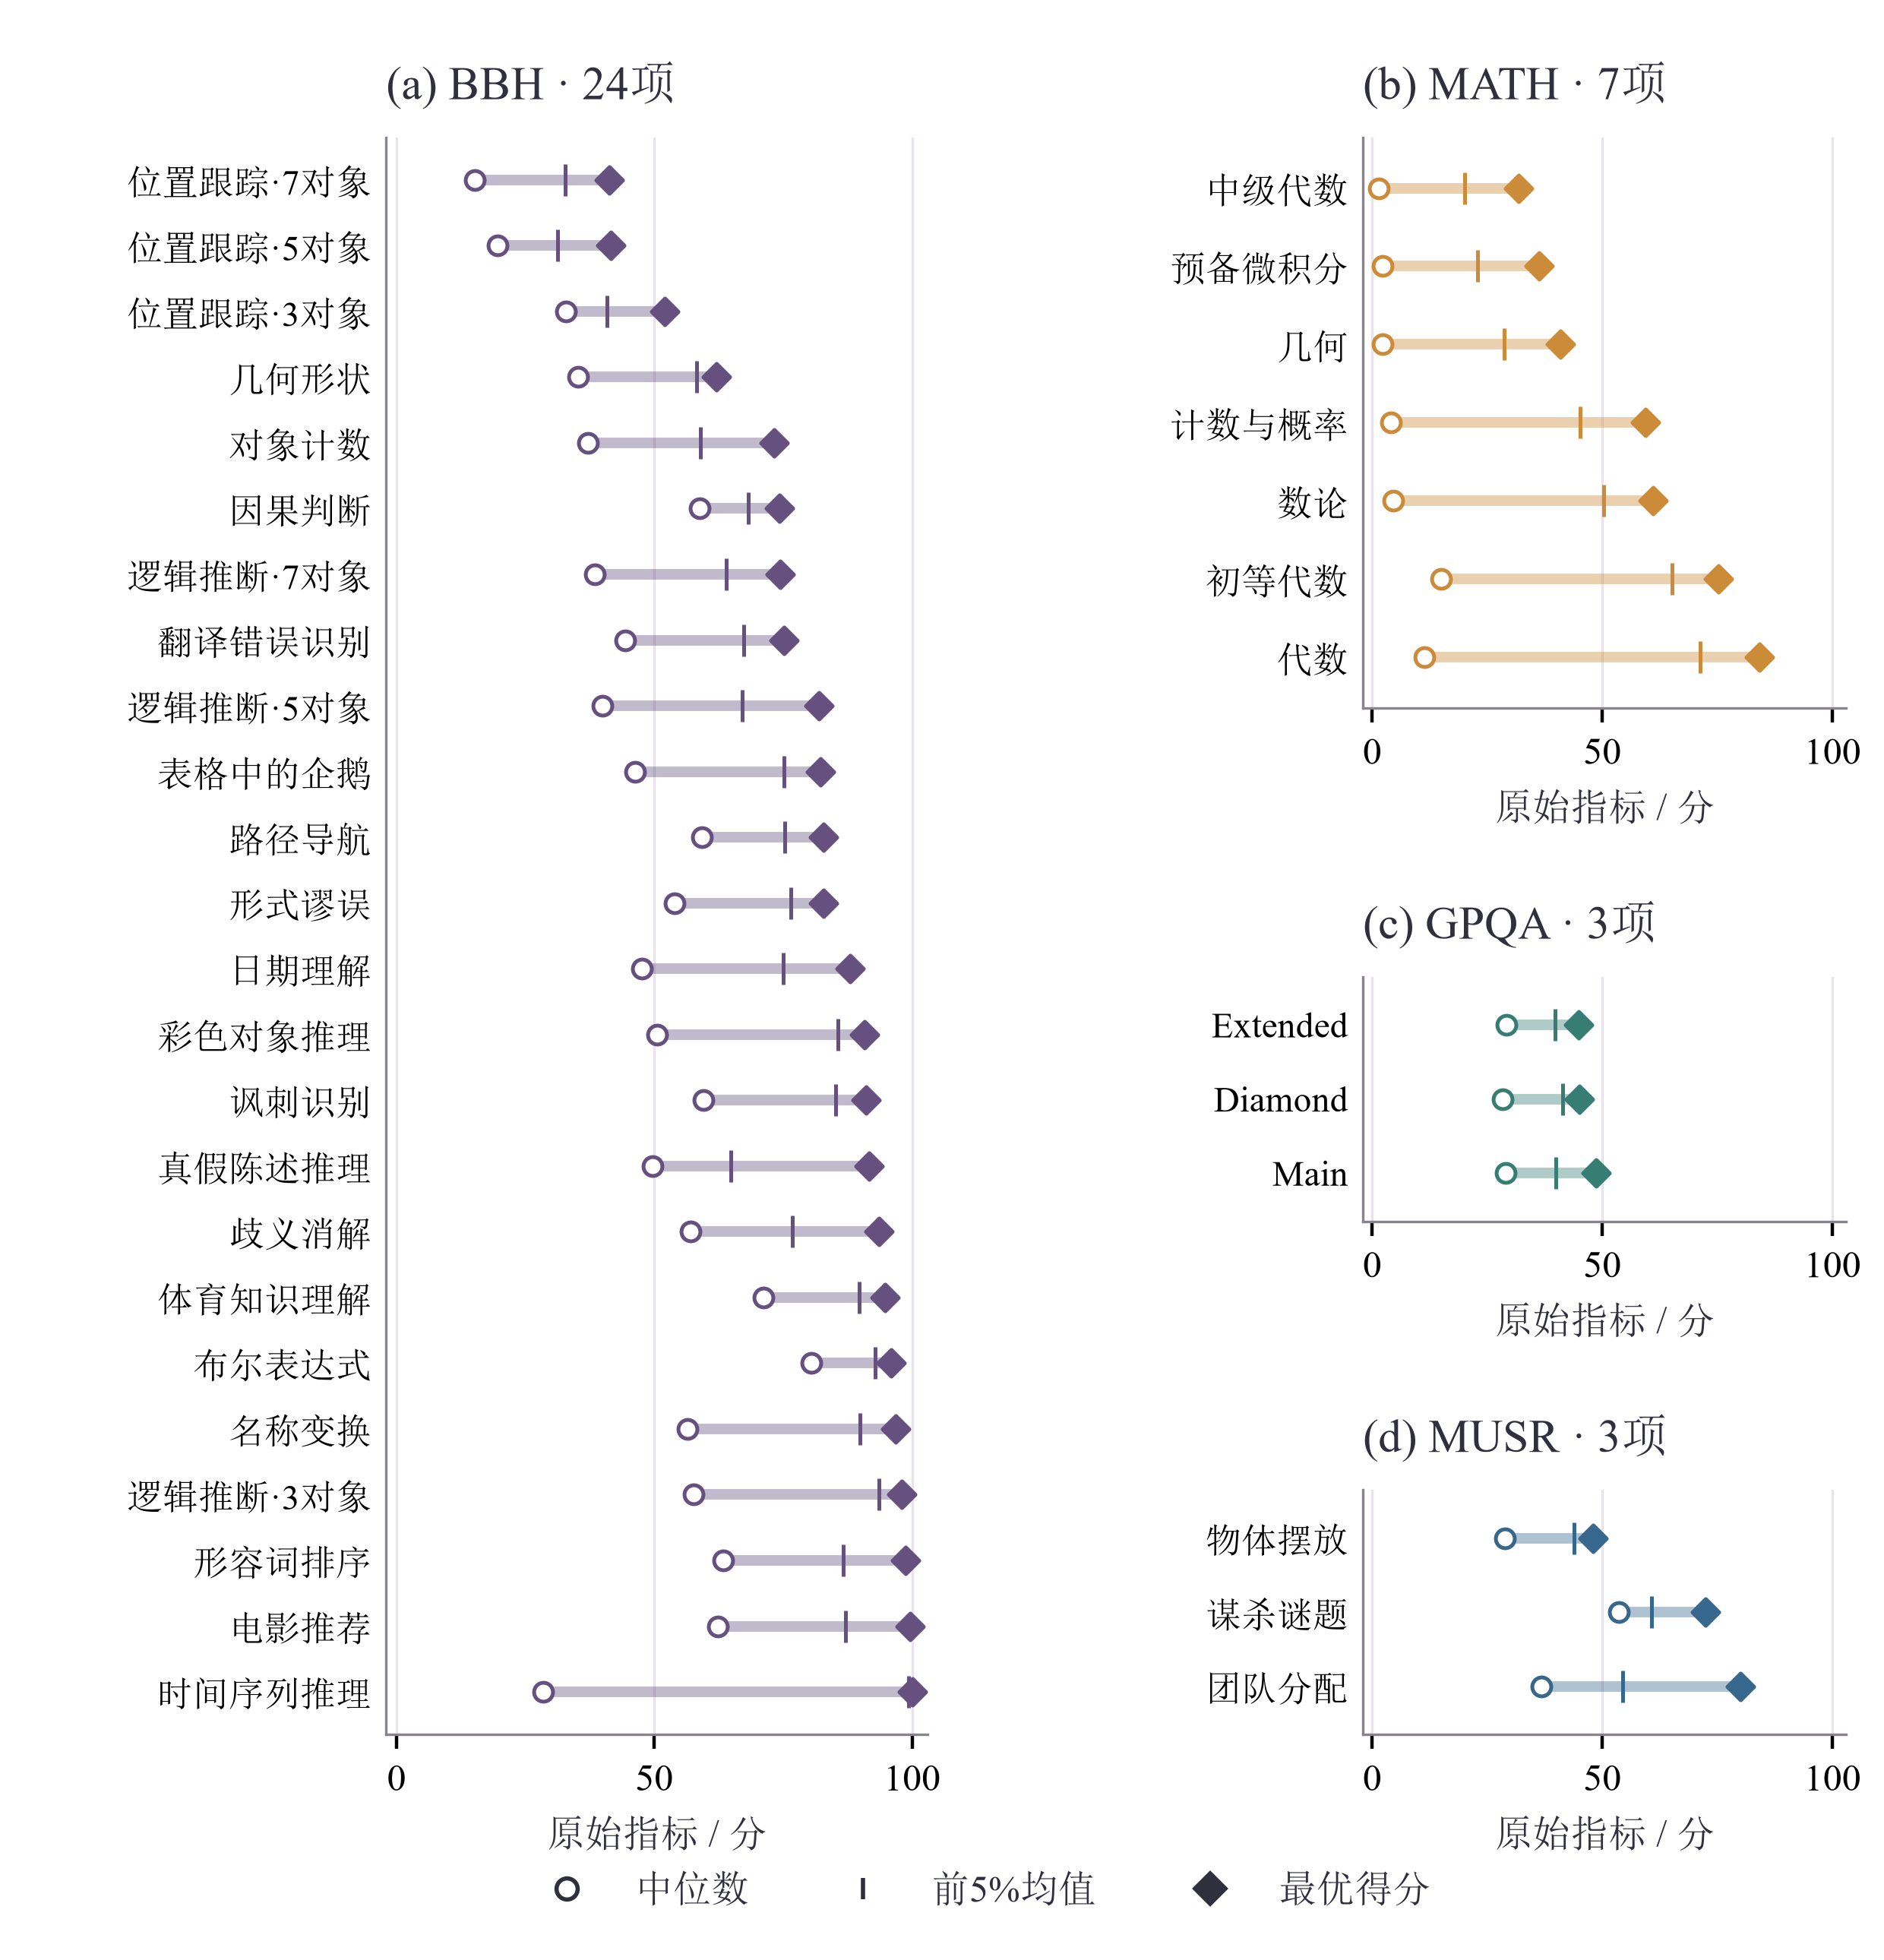
\includegraphics[width=0.98\textwidth]{../求解/问题四/图片/图4_逐任务聚合.png}
\caption{C8 的 37 个子任务表现：圆点、短线和菱形依次为中位数、前 $5\%$ 均值与最优得分；每项 $n=961\sim964$，采用原始指标口径}
\label{fig:p4_task}
\end{figure}

\begin{table}[!htbp]
\centering
\caption{距满分差值最大的六个子任务}
\label{tab:p4_sub}
\begin{tabularx}{0.98\textwidth}{@{}
>{\hsize=0.8\hsize\linewidth=\hsize\raggedright\arraybackslash}X
>{\hsize=2\hsize\linewidth=\hsize\raggedright\arraybackslash}X
>{\hsize=0.6\hsize\linewidth=\hsize\centering\arraybackslash}X
>{\hsize=0.9\hsize\linewidth=\hsize\centering\arraybackslash}X
>{\hsize=0.85\hsize\linewidth=\hsize\centering\arraybackslash}X
>{\hsize=0.85\hsize\linewidth=\hsize\centering\arraybackslash}X@{}}
\toprule
所属类别 & 子任务 & $n$ & \makecell{前 $5\%$\\均值} & 最优得分 & \makecell{距满分\\差值 / 分} \\
\midrule
MATH & 中级代数 & 962 & 20.11 & 31.79 & 68.2 \\
MATH & 预备微积分 & 962 & 22.89 & 36.30 & 63.7 \\
MATH & 几何 & 962 & 28.72 & 40.91 & 59.1 \\
BBH & 位置跟踪，7 个对象 & 964 & 32.67 & 41.20 & 58.8 \\
BBH & 位置跟踪，5 个对象 & 964 & 31.24 & 41.60 & 58.4 \\
GPQA & Extended 子集 & 961 & 39.74 & 44.87 & 55.1 \\
\bottomrule
\end{tabularx}
\end{table}

具体任务中，MATH-Hard 的中级代数、预备微积分和几何最高分在 $31.8\sim40.9$ 之间；BBH 的 5、7 对象位置跟踪约为 41 分；GPQA Extended 为 44.9 分。即便看各项最高表现，这些任务也仍有较大差距，可作为后续改进的关注对象。不过，各任务随机基线和难度不同，不能把原始分数当作完全相同的能力刻度。

按类别汇总，MATH 各任务最高分的均值为 55.5，全部模型和子任务观测合并后的中位数为 3.7；BBH 分别为 81.8、48.8。最高分均值可能由不同模型贡献，不表示某个模型同时达到这些值。结合任务内的分布，可以看出普通表现与单项前沿仍有差距，而不需要假定各任务的得分分布相同。

\subsubsection{宏观资源证据与预测边界}

最后使用 Epoch AI 数据库 C4\cite{epoch2025}观察训练算力、数据量及开放权重状态。它与 C1 规范化名称后只有 1 条匹配，无法组成有效的逐模型联合样本，因此单独用于宏观分析。图\ref{fig:p4_c4}依次给出 Language 领域年度算力范围、开放权重标记比例和 C4 全量字段覆盖，分别说明资源变化和资料完整性。

\begin{figure}[!htbp]
\centering
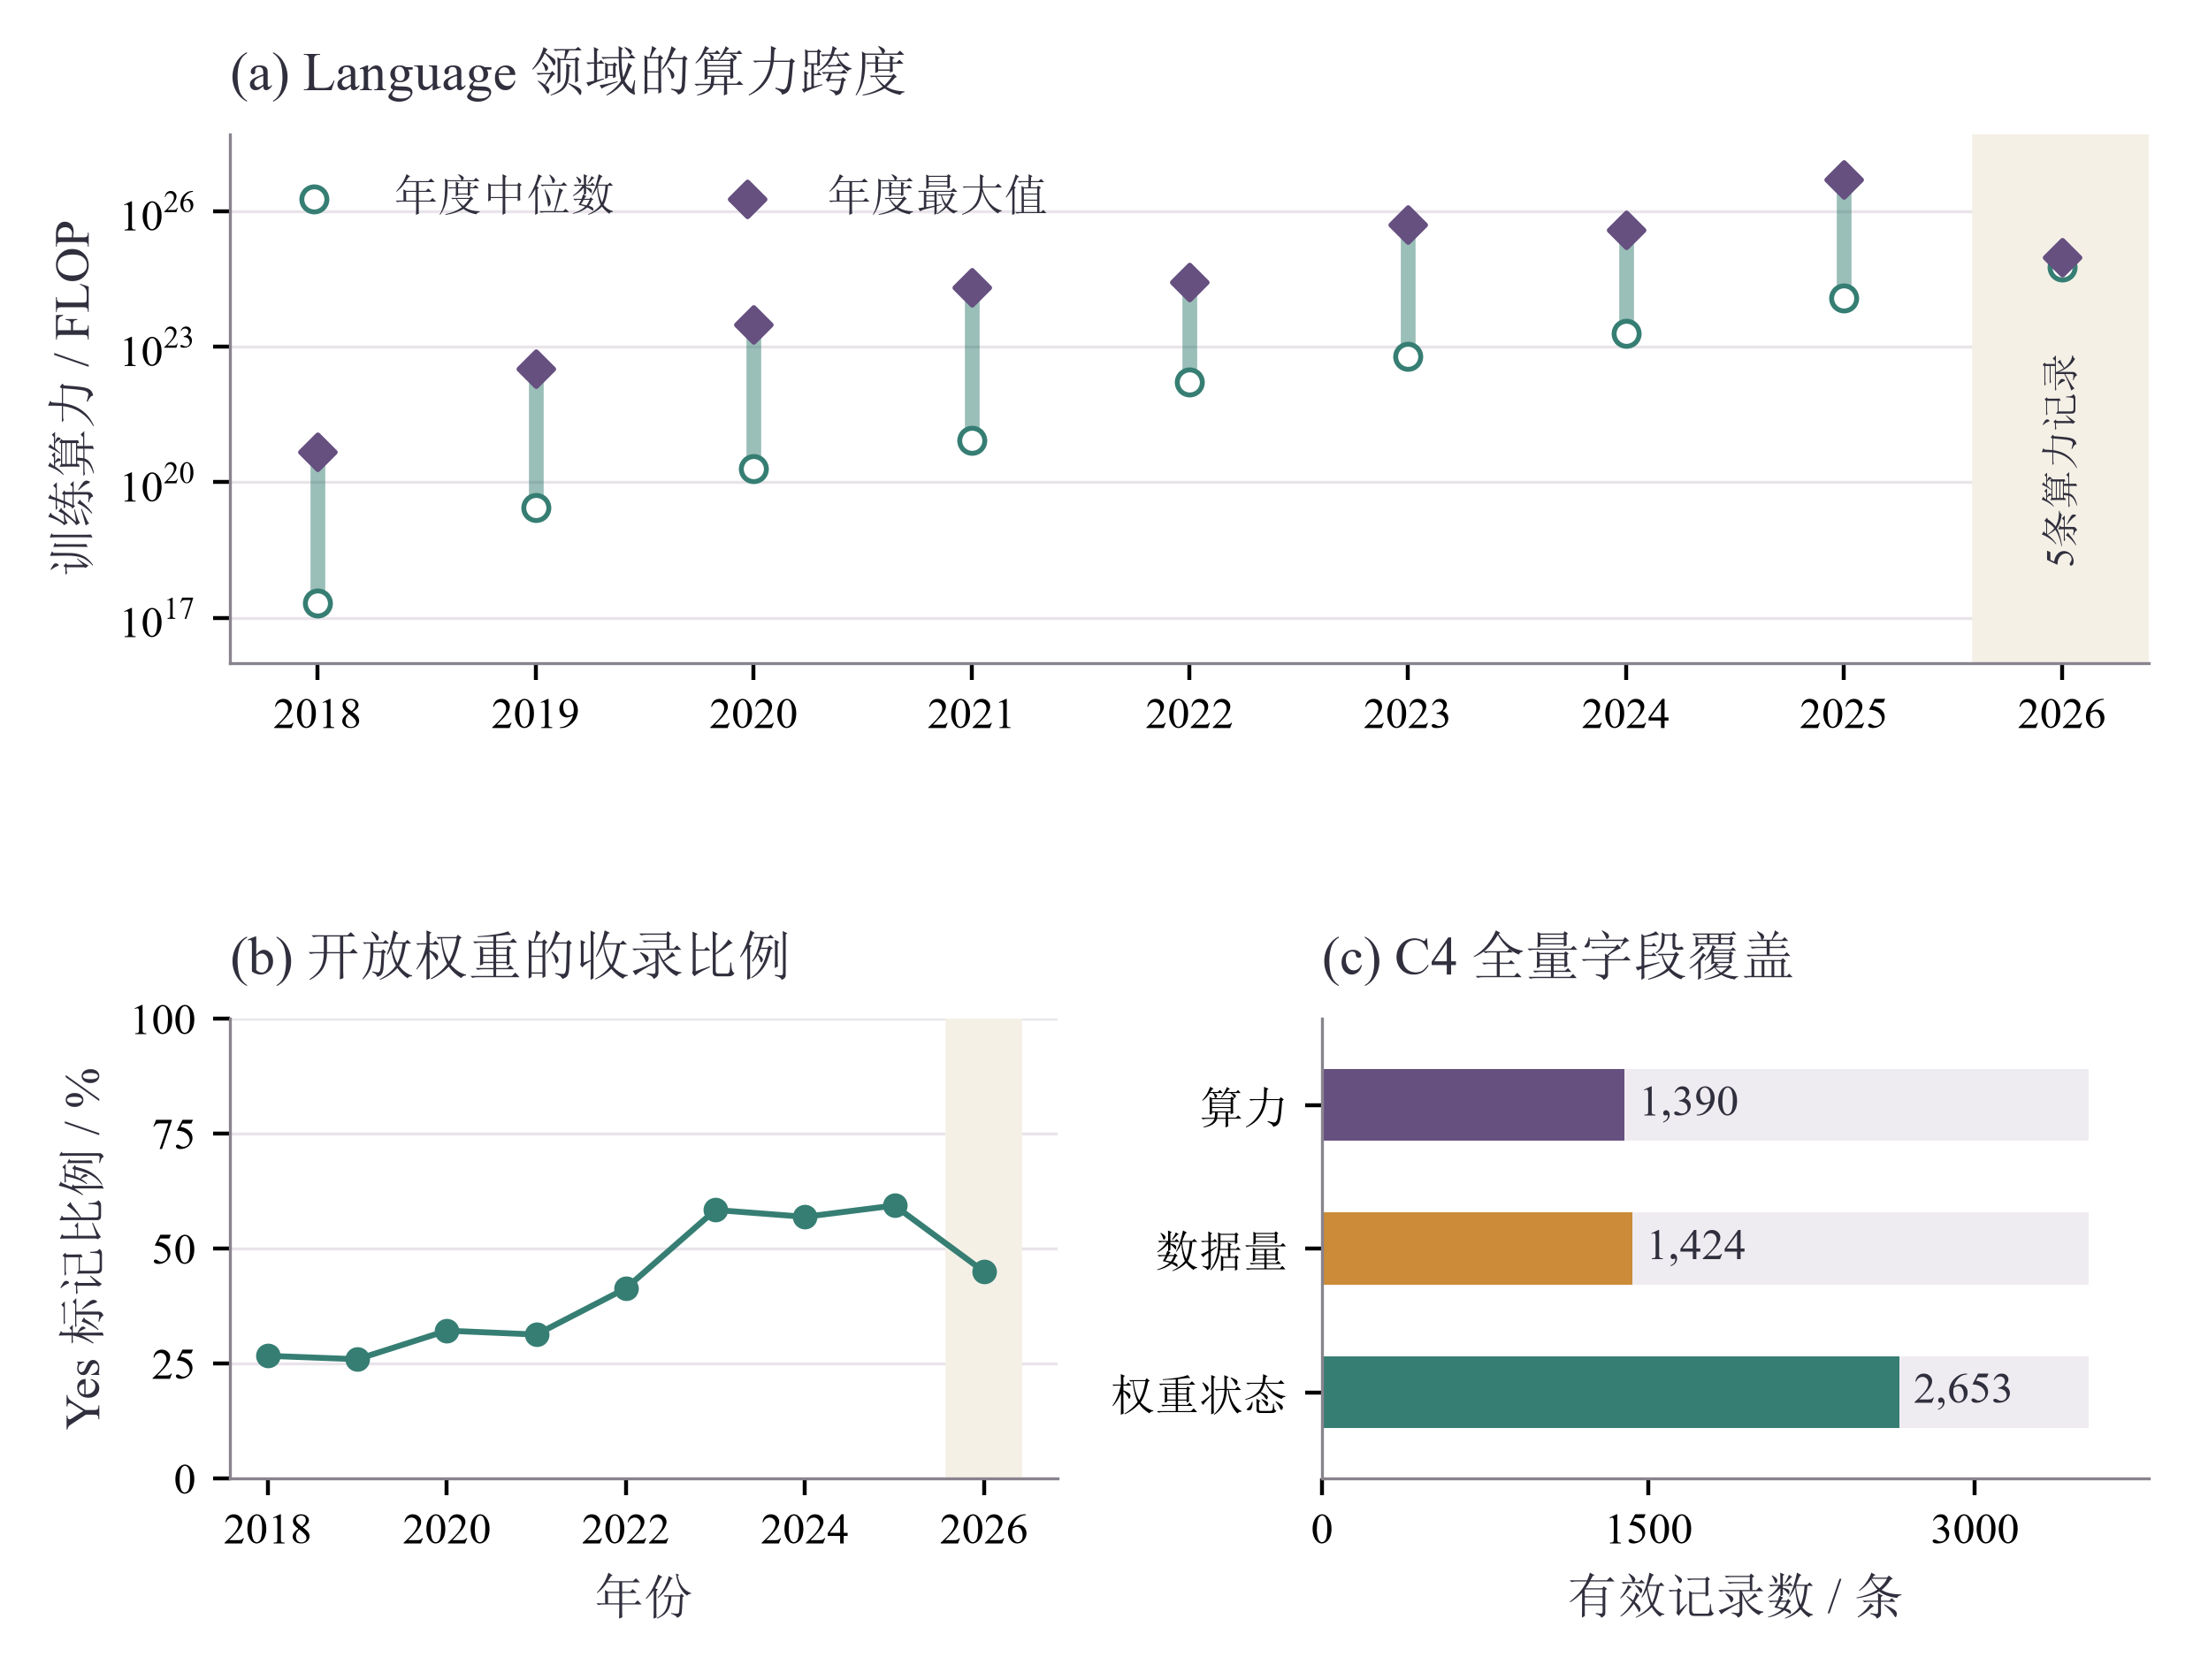
\includegraphics[width=0.98\textwidth]{../求解/问题四/图片/图5_C4宏观趋势.png}
\caption{C4 的资源演进与字段覆盖：上图连接每年算力中位数与最大值；左下为 Language 记录中权重标记 Yes 的比例；右下以全量 3{,}523 条记录为背景，浅色部分为字段缺失或状态未明确}
\label{fig:p4_c4}
\end{figure}

2018 至 2026 年，Language 子集共有 1{,}783 条记录。对九个年度的最大算力取对数拟合，年斜率约为 0.589 个数量级，即相邻年度的拟合算力之比约为 3.88。整体呈扩张趋势，但并不逐年增加，2024 年最大值低于 2023 年。2026 年目前只有 40 条 Language 记录，其中 5 条有算力值，该点容易受到收录不足影响，不能仅凭下降就判断技术趋势逆转。

Language 记录中，开放权重标记 Yes 的占比从 2018 年 26.7\% 变为 2025 年 59.4\%，中间也有下降。计算分母包含当年所有 Language 记录，其中包括权重状态缺失者。因此，该比例反映数据库的收录情况，不等于市场份额，也不足以证明 C1 对总体具有代表性。

C4 全量为 3{,}523 条，其中算力有值的为 1{,}390 条，训练数据量有值的为 1{,}424 条；权重状态明确的 2{,}653 条中，Yes 为 1{,}325，No 为 1{,}328。由于训练数据量缺失较多、来源也不统一，本节只报告其覆盖情况，不另估年度增长率。宏观变化可以帮助设置不同资源情景，但还不能确定算力放缓会使非规模进步按什么比例下降。

本问先确认了损失与能力之间的方向性联系，再分别核算长期和近期的前沿增量。长期样本中规模与非规模项大致各占一半，2024 年 6 至 9 月则主要为非规模项，两者需要按各自样本解释。未来预测同时保留曲线区间和结构情景的差异；具体能力改进则可重点观察数学、研究生级问答和多步推理等薄弱任务。

\FloatBarrier
\endgroup
